\documentclass[12pt,openbib]{beamer}

\author{Pritvi Jheengut @zcoldplayer} %\thanks{\and}}
\title{An introduction to The seL4 MicroKernel}
\subtitle{Learn about the secure and performant MicroKernel}
\subject{Oye}

\usepackage[size=custom,width=64,height=36,orientation=landscape,
  scale=1.75]{beamerposter}

\usepackage{lmodern}
\usepackage[T1]{fontenc}
\usepackage[utf8]{inputenc}

% Eliminate errors such as
% \LaTeX\ Font Warning: Font shape `T1/cmss/m/n' in size <4> not available
% \LaTeX\ Font Warning: Size substitutions with differences up to 1.0pt

\usepackage{hyperref}
\hypersetup{
  pdfcreator=pdflatex,
  pdffitwindow=true
}

\usepackage{verbatim}

\usepackage[french,UKenglish]{babel}
\usepackage{listings}

% \usepackage{pgf}
% \usepackage{xy}[all]
\usepackage{graphicx}

\usepackage{tikz}
\usetikzlibrary{shapes.geometric, arrows,positioning}

\usepackage{smartdiagram}

% \usepackage{booktabs}

% usetheme{DevConMU2019}

\mode<presentation>

  \useoutertheme{infolines}

  \definecolor{light}{HTML}{0088FF}
  \definecolor{confblue}{HTML}{111144}
  \definecolor{confred}{HTML}{771111}
  \definecolor{confyellow}{HTML}{FF5533}

  \setbeamercolor{alerted text}
  {bg=confblue,fg=-confyellow}

  \setbeamercolor{block title}
  {bg=confred!95,fg=white}

  \setbeamercolor{block body}
  {bg=confblue!95,fg=confyellow}

  \setbeamercolor{frametitle}
  {parent=confyellow,fg=confyellow!35}

  \setbeamercolor{normal text}
  {bg=confblue,fg=confyellow}

  \setbeamercolor*{palette primary}
  {use=structure,fg=confblue,bg=structure.fg}

  \setbeamercolor*{palette secondary}
  {use=structure,fg=confblue,bg=structure.fg!85!-confblue}

  \setbeamercolor*{palette tertiary}
  {use=structure,fg=confblue,bg=structure.fg!70!-confblue}

  \setbeamercolor{structure}
  {bg=-confblue,fg=light!75}

  \setbeamercolor{Title bar}
  {fg=confred!90}

  \setbeamercolor{titlelike}
  {parent=-confyellow,bg=structure.fg!30!-confyellow,fg=black!85}

  \setbeamercovered{transparent,dynamic}

  \setbeamersize{text margin left=8cm,text margin right=2cm}

  \setbeamertemplate{blocks}[rounded][shadow=true]

  \setbeamertemplate{background canvas}[vertical shading]
  [top=confred,middle=confblue,bottom=confred!75]

  \setbeamertemplate{sidebar canvas left}{

    \vspace{6cm}

    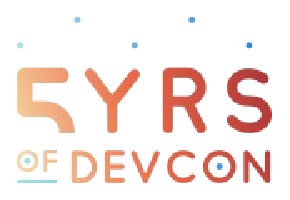
\includegraphics[width=30cm,height=48cm]{5years.eps}

    \vspace{-32cm}

    \includegraphics[width=8.4cm,height=8cm]{mscc.eps}

  }

% \mode<handout>{\beamertemplatesolidbackgroundcolor{black!50}}

\mode<all>

\begin{document}

\section{Title : Presentation for \#DevConMU}

\frame{
  \frametitle{Developers Conference \#DevConMU \\ @ the Voila Hotel
    \&  Flying Dodo}

  \huge
  \maketitle

}

\section{}
\section{Intellectual Property Alert : Overview of the Copyleft
  Licenses}

\frame{
  \frametitle{Copyleft License Attribution}

  Made with love using beamer, \LaTeX\ and git.\\
  You can view at
  \href{https://github.com/Pritvi-DevConMU-MSCC/Introduction2seL4}
  {Introduction to seL4}

  \begin{alertblock}{This work is licensed under the \LaTeX\ Project
      Public License.}
    To view a copy of this license, visit \\
    \url{https://www.latex-project.org/lppl.txt}
  \end{alertblock}

  \begin{alertblock}{This work is licensed under the Creative
      Commons Attribution-ShareAlike 4.0 International License.}
    To view a copy of this license, visit \\
    \href{http://creativecommons.org/licenses/by-sa/4.0/}{CC BY-SA}
    or \\

    send a letter to \\
    Creative Commons, \\
    PO Box 1866, \\
    Mountain View, \\
    CA 94042, \\
    USA. \\
  \end{alertblock}

}

\section{Greetings}
\subsection{About the Author}

\frame{
  \frametitle{Who Am I}

  \large

  \href{http://slackware.com/}{Geek@Slackware}

  \href{https://twitter.com/zcoldplayer}{twitter @zcoldplayer}

  \href{https://xmail.net/z.coldplayer}{zcoldplayer xmail Website}

  \href{http://metservice.intnet.mu/}{Work
    : SMTT@Meteorological.Services.mu}

  Active in many User group LUGM, MMC, MSCC, FECM, GDG\_MU \\
  and several other hackathons

  Passionate about how and why things work.

  Fervour Advocate of Free Libre and Open Source Software.

}

\subsection{About the Audience}

\frame{
  \frametitle{Who are you}

  \large

  \begin{block}{Would you mind tell me who you are?}
    Some hints:
  \end{block}

  \begin{enumerate}
  \item @twitter\_handle
  \item where you work
  \item email you want to share
  \item Hobbies
  \item purpose and expectations of this session
  \end{enumerate}

}

\section{Community Groups in Mauritius}

\frame{
  \frametitle{Community Groups in Mauritius}

  \begin{block}{Healthy growth of Community Groups in Mauritius}
    This turn of the century has seen an uprising of Community groups
    in Mauritius in the field of the Digital World. The diversity has
    helped the exchange and sharing of innovative ideas, experience,
    bleeding edge technology, upcoming events, conferences in the
    Digital Island of the Republic of Mauritius.
  \end{block}

  This is a list of some of the active communities in Digital
  Mauritius.

  \begin{itemize}
  \item Linux User Group Meta, LUGM
  \item Mauritius Software Craftsmanship Community, MSCC
  \item Mauritius Makers Community, MMC
  \item Front-End Coders Mauritius, FECM
  \item PHP User Group of Mauritius, phpMauritiusUG
  \item Symfonymu
  \item Google Developers Group Mauritius, GDG\_M
  \item Digital Marketing Mauritius
  \end{itemize}

}

\section{The Kernel}

\begin{frame}

  \frametitle{Underlying OS basics}

  \begin{block}{What Do You Understand By An Operating System ?}

    \begin{itemize}
    \item<1> Provide The User Utilities, Programs to perform jobs
    \item<2> Manage the Hardware on which it is running
    \item<3> Manage resources automatically
    \item<4> The OS and the hardware together is called a Computer
    \end{itemize}

  \end{block}

  An Operating System contains a Kernel, the Kernel is not an OS.

\end{frame}

\subsection{A bridge}

\frame{
  \frametitle{The importance of the Kernel}

  \begin{block}{In Computer science}

    \begin{center}
      the Kernel is the bridge between \\
      the hardware and user space Software \\
      as shown in a hierarchical protection domain system.

    \end{center}

  \end{block}

  \begin{center}
    \begin{tikzpicture}

      \tikzstyle{startstop}=[rectangle,rounded corners,
        minimum width=20cm,minimum height=2cm,
        text centered,fill=darkgray!90]

      \node(HARDWARE1)[startstop]{HARDWARE};
      \node(Kernel1)[startstop,below =of HARDWARE1,
        yshift=-3cm]{Kernel};
      \node(SOFTWARE1)[startstop,below =of Kernel1,
        yshift=-3cm]{USER END SOFTWARE};

      \draw [line width=0.25cm,<->,lime]
      (HARDWARE1)--(Kernel1);
      \draw [line width=0.25cm,<->,lime]
      (Kernel1)--(SOFTWARE1);

      \node(HARDWARE2)[startstop,below right=of HARDWARE1,
        yshift=3cm]{HARDWARE SPACE};
      \node(Kernel2)[startstop,below right=of Kernel1,
        yshift=3cm]{Kernel SPACE};
      \node(SOFTWARE2)[startstop,below right=of SOFTWARE1,
        yshift=3cm]{USER SPACE};

      \draw [line width=0.25cm,<->,lime]
      (HARDWARE2)--(Kernel2);
      \draw [line width=0.25cm,<->,lime]
      (Kernel2)--(SOFTWARE2);

    \end{tikzpicture}

  \end{center}

}

\subsection{Different Role undertaken}

\frame{
  \frametitle{Multi functionality of the Kernel}

  \begin{block}{The Kernel in general manages resources such as :}

    \begin{itemize}
    \item Processing and Memory units
    \item Process Capabilities and Virtual addressing
    \item Input as well as Output Devices
    \item Virtualisation and by extension Containers
    \item Access Control lists, Security and Cryptographic Mechanisms
    \end{itemize}

  \end{block}

}

\subsection{Hardware abstraction}

\frame{
  \frametitle{Hardware abstraction layers of the Kernel}

  \begin{block}{The Kernel provides hardware abstraction}

    \begin{center}

      for the underlying user space software using hierarchical
      protection domains.

    \end{center}

    Hardware abstraction is crucial in cases such as

    \begin{itemize}
    \item portability
    \item security frameworks
    \item code reuse
    \item forward and backward version compatibility
    \item fault tolerance
    \end{itemize}

    A Kernel once built, can be run on several different types of
    platform but of similar architectures.

  \end{block}

}

\subsection{Different scenario of a running Kernel}

\frame{
  \frametitle{The Multi Tasking Approach using a Kernel}

  \begin{block}{Scheduling processes}

    In a multi tasking environment, process scheduling is
    primordially managed by the Kernel.

    A process contains both
    \begin{itemize}
    \item Data
    \item Instruction
    \end{itemize}

    Mechanisms provided by the Kernel manage processes using

    \begin{itemize}
    \item Overall performance or system load
    \item CPU and Memory as well as Networking usage
    \item Input and Output Device Isolation
    \item ACL's and Capabilities
    \end{itemize}

  \end{block}

}

\frame{
  \frametitle{Example of Scheduling Processes}

  \begin{block}{A prime example of the Kernel's role in this context
      is to separate processes resources so that}

    \begin{itemize}
    \item one process do not overwrite or read another's process
      data either in
      \begin{enumerate}
      \item Volatile Memory or
      \item Persistent Storage
      \end{enumerate}
    \item one process is not utilising greedily the CPU, network,
      memory continuously at the expense of other processes
    \item regulate Input and Output Devices with the respective
      process
    \item The overall performance of the system is within the
      permissive set limits
    \end{itemize}

  \end{block}

  There exist several implementations of all these Mechanisms,
  hierarchical protection domains, Capabilities set with the hardware
  or provided by the Kernel or inherited by the processes through
  software libraries provided by the Operating System as a whole.

}

\subsection{Major Kernel Design}

\frame{
  \frametitle{The major Kernel Design Implementations}

  \begin{center}

%     \smartdiagramset{text color = white}

    \smartdiagram[bubble diagram]{
      \textbf{Implementations} \\ \textbf{and Design} \\
      \textbf{Approach},
      \textbf{Monolithic} \\ \textbf{Kernel},
      \textbf{Hybrid} \\ \textbf{Kernel},
      \textbf{$\mu$K} \\ \textbf{ MicroKernel} }

  \end{center}
}

\subsection{The Monolithic Kernels}

\frame{
  \frametitle{The Most famous Monolithic Kernel in the world}

  \begin{block}{\url{https://www.Kernel.org} : The home of the Linux
      Kernel}

    Linux is GPL'ed Freely licensed Monolithic Kernel developed by
    Linus Torvalds who also is the creator of git.

  \end{block}

  \begin{block}{Inspired by the $\mu$Kernel Minix as a Unix Clone,}
    Linux was initially publicly released in 1991 primed for the
    relatively cheap x86 based IBM clone PC.

    Being Monolithic, Linux contains all the previously mentioned
    Capabilities and Mechanisms inside the Kernel all running within
    the Kernel Space

  \end{block}

}

\frame{
  \frametitle{The Most famous Monolithic Kernel in the world}

  \begin{alertblock}{Linux is Everywhere}

    Our Benevolent Dictator, Lord Linus dreamed of conquering the
    world and he achieved it.

    \begin{itemize}
    \item Most Smart

      \begin{enumerate}
      \item Phones
      \item TV
      \item Cars
      \item Guns
      \item Camera
      \end{enumerate}

      runs Tizen, Android and Firefox OS/KaiOS or in another Form.
    \item All of Top 500 Supercomputers runs Linux since two years
    \item Ported to most architectures
    \item Powers 80\% - 90\% of the Internet and most of the
      cloud
    \item Intensive and highly complex CGI are produced by Linux
      Clusters
    \end{itemize}

  \end{alertblock}

  \begin{block}{Except the Desktop}
    even steam accounts for almost 1\%
  \end{block}

}

\frame{
  \frametitle{less famous Monolithic Kernels}

  Other dominant Monolithic Kernels
  \begin{itemize}
  \item The BSD Family :: FreeBSD, NetBSD, OpenBSD
  \item MS-DOS / FreeDOS
  \item Unix System V based OS :: AIX, HP-UX, Solaris
  \end{itemize}

  \begin{block}{FreeBSD is Open Licensed as such as the other BSD's}

    Therefore, it can used in closed source hardware such as

    \begin{itemize}
    \item Routers, Switches, Firewalls
    \item PS4
    \item Windows Network stack
    \item Components of them are used in other software
    \end{itemize}

  \end{block}

}

\subsection{Issues with Monolithic Kernels}

\frame{
  \frametitle{The Hierarchical protection Domain Design of
    Monolithic Kernel}

  \begin{block}{Use case of the Hierarchical protection Domain}

    Improves granularity in addition to the robustness of protective
    mechanisms by separating all Kernel services in Kernel space and
    the remaining unprivileged services in user space.

  \end{block}

  \begin{center}
    \begin{tikzpicture}

      \tikzstyle{startstop}=[rectangle,rounded corners,
        minimum width=20cm,minimum height=2cm,
        text centered,fill=darkgray!90]

      \node(Kernel1)[startstop]{Kernel SPACE};
      \node(SOFTWARE1)[startstop,below =of Kernel1,
        yshift=-0.5cm]{USER SPACE};

      \draw [line width=0.25cm,<->,lime]
      (Kernel1)--(SOFTWARE1);

      \node(Kernel2)[startstop,below right=of Kernel1,
        yshift=3cm]{Kernel};
      \node(SOFTWARE2)[startstop,below right=of SOFTWARE1,
        yshift=3cm]{END USER SOFTWARE};

      \draw [line width=0.25cm,<->,lime]
      (Kernel2)--(SOFTWARE2);

    \end{tikzpicture}

  \end{center}

  \begin{block}{Inside the Kernel space or Supervisor mode, everything
      is possible}

    The Kernel provides System Calls for user
    software in order to permit them to perform privileged operations

  \end{block}

  \begin{block}{Inside the user space, the protected domain permits
      only safe operations and unprivileged actions are permitted}

    When a user space process tries to directly access a Kernel space
    process, a protection fault exception is reported by the Kernel.

  \end{block}

}

\frame{
  \frametitle{If Monolithic Kernels Work, then where is the Issue?}

  \begin{block}{In general, Monolithic Kernels are}

    \begin{itemize}
    \item very big, sometimes in the dozens of Megabytes
    \item difficult to Maintain
    \item licensing issues with third party partners, vendors
    \item
    \item hard to detect and eliminate bugs in general
    \item not much extensible
    \item resource and time consuming for new compilations
    \end{itemize}

  \end{block}

  To address these issues, one solution major Operating System
  vendors have adopted is Hybrid Kernels.

  The other solution is $\mu$Kernels.

}

\subsection{Hybrid Kernels}

\frame{
  \frametitle{Some common Hybrid Kernels in the Market}

  \begin{block}{}

    Some Hybrid Kernels include

    \begin{itemize}
      \item \href{https://en.wikipedia.org/wiki/XNU}{Apple Kernel}
      \item \href{https://en.wikipedia.org/wiki/Architecture_of_Windows_NT
      }{Microsoft Windows NT kernel}
    \end{itemize}


  \end{block}

}

\subsection{MicroKernels}

\frame{
  \frametitle{The $\mu$Kernel}

  \begin{block}{What is a $\mu$Kernel ?}

    By moving all non-essential services, protocol stack, file system
    management, device driver stack out of the Kernel space into the
    user space, the size of the Kernel code reduces dramatically such
    that certain Kernels can fit into the Level one cache of CPU's.

  \end{block}

  \begin{center}
    \begin{tikzpicture}

      \tikzstyle{startstop}=[rectangle,rounded corners,
        minimum width=10cm,minimum height=3cm,
        text centered,fill=darkgray!90]

      \node(Kernel1)[startstop]{Kernel SPACE};
      \node(SOFTWARE1)[startstop,below =of Kernel1,
        yshift=-7cm]{USER SPACE};

      \draw [line width=0.25cm,<->,lime]
      (Kernel1)--(SOFTWARE1);

      \node(Kernel2)[startstop,below right=of Kernel1,
        yshift=4cm,xshift=10cm]{$\mu$Kernel};
      \node(STACK1)[startstop,below right=of SOFTWARE1,
        yshift=5cm]{Interprocess Protocol};
      \node(STACK2)[startstop,below right=of STACK1,
        yshift=4cm]{FileSystems};
      \node(STACK3)[startstop,below right=of STACK2,
        yshift=4cm]{Device Driver};
      \node(STACK4)[startstop,below =of STACK3,
        yshift=2cm]{Process \& Memory manager};
      \node(SOFTWARE2)[startstop,below =of STACK1,
        yshift=-2cm,xshift=6cm]{END USER SOFTWARE};

      \draw [line width=0.25cm,<->,lime]
      (Kernel2)--(SOFTWARE2);
      \draw [line width=0.25cm,<->,lime]
      (Kernel2)--(STACK1);
      \draw [line width=0.25cm,<->,lime]
      (Kernel2)--(STACK2);
      \draw [line width=0.25cm,<->,lime]
      (Kernel2)--(STACK3);
      \draw [line width=0.25cm,<->,lime]
      (Kernel2)--(STACK4);

    \end{tikzpicture}

  \end{center}

}

\frame{
  \frametitle{The $\mu$Kernel}

  \begin{block}{The $\mu$Kernel advantages with respect to
      Monolithic Kernels}

    This brings some advantages such as ::

    \begin{itemize}
    \item smaller size means code gets to run more rapidly
    \item security is enhanced by having minimal dependencies and
      code review is improved too
    \item Maintenance becomes easy on the long run
    \item Feature extension is not an issue at the user space
    \item easy to have third party vendor components with complying
      licenses
    \item small code means bug detection is not that hard at all
    \item compilation of a new Kernel involves minimal resources
      and takes a small time to fulfil
    \end{itemize}

  \end{block}

}

\section{seL4 - The MicroKernel}

\subsection{Introduction to some MicroKernels}

\frame{
  \frametitle{The Mach $\mu$Kernel Family}

  \begin{block}{Mach is a kernel developed at Carnegie Mellon
      University}
    to support operating system research, primarily distributed and
    parallel computing.

    Mach is often mentioned as one of the earliest examples of a
    microkernel

  \end{block}

  \begin{block}{IPC overhead is a major issue for Mach 3 systems}

    This issue has been one of the reason $\mu$Kernel has a bad
    reputation in the industry.

    A single-side of a syscall took \href{http://www.lemis.com/papers/Taiwan/tutorial.pdf
    }{20$\mu$s} under BSD and \href{https://www.cscjournals.org/manuscript/Journals/IJE/Volume5/Issue4/IJE-294.pdf
    }{114$\mu$s} on Mach running on the same system.

  \end{block}

}

\frame{
  \frametitle{The L4 $\mu$Kernel Family}

  \begin{block}{L4 created by Jochen Liedtke is a family of
      second-generation microkernels}

    \begin{itemize}
    \item useful to implement Unix-like Operating Systems
    \item designed from the start for

      \begin{enumerate}
      \item high performance
      \item improving security
      \item isolation
      \item robustness
      \end{enumerate}

    \end{itemize}

  \end{block}

}

\subsection{About seL4 and its advantages}

\frame{
  \frametitle{About seL4}

  \href{http://ts.data61.csiro.au/projects/seL4/}{sel4}
  is a $\mu$Kernel.

  \begin{block}{\url{http://sel4.systems/}}

    The world's first operating-system kernel with \href{http://sel4.systems/Info/Docs/GD-NICTA-whitepaper.pdf
    }{an end-to-end proof} of \href{http://ts.data61.csiro.au/projects/seL4-verification/
    }{implementation correctness and security enforcement} is
    available as open source.

    sel4 has been proved with
    \begin{itemize}
     \item Functional correctness
     \item Integrity and information flow security
     \item Compilation correctness
     \item Verified worst-case execution time
    \end{itemize}

  \end{block}

  More information about seL4 is available \href{https://www.cse.unsw.edu.au/~cs9242/18/lectures/07-ukinternals.pdf
  }{here} and \href{https://securityaffairs.co/wordpress/27087/hacking/sel4-hack-proof-darpa-derived-micro-kernel-goes-open-source-tomorrow.html
  }{here.}

}
%
\frame{
  \frametitle{github and seL4}
%
  \href{https://github.com/seL4}{seL4 Howto and repositories}

  \begin{block}{github}

    \begin{itemize}
      \item \href{https://docs.sel4.systems/GettingStarted.html}{
      How to start with seL4}
    \item \href{https://github.com/seL4/util_libs}{utils for seL4}
    \item \href{https://docs.sel4.systems/UserlandComponents.html
    }{Userland Components and Drivers}
    \item \href{https://docs.sel4.systems/CAmkES/}{CAmkES}
    \end{itemize}

  \end{block}

    \begin{block}{CAmkES}

      CAmkES is a component architecture for microkernel-based
      embedded systems is a software development and runtime
      framework for quickly and reliably building microkernel-based
      multiserver systems.

  \end{block}
}

\subsection{Case use of seL4}

\frame{
  \frametitle{seL4 in practice}


  \begin{block}{\href{https://docs.sel4.systems/Hardware/
      }{Hardware support of seL4}}

    \begin{itemize}
      \item \href{https://www.hardkernel.com/}{Odroid XU4}
      \item \href{https://www.raspberrypi.org/}{Raspberry Pi}
      \item \href{https://beagleboard.org/}{Beagle Board}
    \end{itemize}


  \end{block}

  \href{https://research.csiro.au/tsblog/
  }{Data61’s Trustworthy Systems Research Group} is one of the
  companies who actively develop seL4.

}

\frame{
  \frametitle{Questions}

  \huge

  \begin{center}

    QUESTIONS!

  \end{center}

}

\end{document}
